\documentclass[12pt]{article}
\usepackage[utf8]{inputenc}
\usepackage{amsmath}
\usepackage{soul}
\usepackage{xcolor}
\usepackage{amssymb}
\usepackage{float}
\usepackage{graphicx}
\usepackage{geometry}
\usepackage{framed} % For the box
\sethlcolor{yellow}
\newcommand{\red}[1]{\textcolor{red}{#1}}
\newcommand{\blue}[1]{\textcolor{blue}{#1}}

% Adjust margins
\geometry{margin=1in}

\title{\textbf{CSE421: Design and Analysis of Algorithms}}
\author{Homework 1 \\ Shaqan Oveis Gharan}
\date{March 27th, 2024 \\ Due: April 3rd, 2024 at 11:59 PM}


\begin{document}

\noindent CS-3510-\textbf{\red{Your Section\#}} Algorithms, Spring 2025\hfill Mid-Term 1 Take-Home\\
\blue{Hayden} \blue{Hawley} \hfill Collaborator(s):

\hrulefill

\subsection*{Problem 1 (10 pts)}
For this problem, we explore the issue of \textit{truthfulness} in the Gale-Shapley algorithm for Stable Matching. Show that a participant can improve its outcome by lying about its preferences. Consider $r \in R$. Suppose $r$ prefers $p$ to $p'$, but $p$ and $p'$ are low on $r$'s preference list. Show that it is possible that by switching the order of $p$ and $p'$ on $r$'s preference list, $r$ achieves a better outcome, e.g., is matched with a $p''$ higher on the preference list than the one if the actual order was used.

\textit{Hint:} Prove the claim by finding one specific instance of stable matching problem and comparing the stable matching before and after the switching.

\subsection*{Solution}

\textbf{Setup.} Let the two sides be:
\[
\text{Residents (receivers)}: R = \{r, s, t\}, 
\quad
\text{Programs (proposers)}: P = \{p, p', q\}.
\]
We run the program-proposing Gale-Shapley algorithm.

\subsubsection*{True Preferences}
\begin{itemize}
    \item \(\text{Resident }r:\quad q \succ p \succ p'\)
    \item \(\text{Resident }s:\quad p \succ q \succ p'\)
    \item \(\text{Resident }t:\quad p \succ p' \succ q\)
    \item \(\text{Program }p:\quad r \succ s \succ t\)
    \item \(\text{Program }p':\quad r \succ t \succ s\)
    \item \(\text{Program }q:\quad s \succ r \succ t\)
\end{itemize}

\subsubsection*{Case 1: $r$ Reports Truthfully}
\begin{enumerate}
    \item \textbf{Round 1.} 
    \begin{itemize}
        \item \(p\) proposes to \(r\). 
        \item \(p'\) also proposes to \(r\). 
        \item \(q\) proposes to \(s\).
    \end{itemize}
    \item \textbf{Resident Decisions.}
    \begin{itemize}
        \item \(r\) receives proposals from \(p\) and \(p'\). 
              Since \(r\)'s true order is \(q \succ p \succ p'\) (and \(q\) did not propose), \(r\) prefers \(p\) over \(p'\). 
              Therefore \(r\) holds \(p\) and rejects \(p'\).
        \item \(s\) holds \(q\). 
        \item \(t\) receives no proposal yet.
    \end{itemize}
    \item \textbf{Round 2.}
    \begin{itemize}
        \item \(p'\) (rejected by \(r\)) proposes to its next choice, \(t\). 
        \item \(t\) accepts \(p'\), having no other offer.
    \end{itemize}
    \item \textbf{Final Matching.}
    \[
    r \leftrightarrow p, \quad s \leftrightarrow q, \quad t \leftrightarrow p'.
    \]
\end{enumerate}

Here, \(r\) ends up with \(p\). Since \(q\) went to \(s\), \(r\) cannot do better under truthful reporting.

\subsubsection*{Case 2: $r$ Misreports by Swapping $p$ and $p'$}
Now suppose \(r\) reverses \(p\) and \(p'\) in his submitted list:
\[
\text{Reported by }r:\quad q \succ p' \succ p.
\]
Then:

\begin{enumerate}
    \item \textbf{Round 1.}
    \begin{itemize}
        \item \(p\) proposes to \(r\).
        \item \(p'\) also proposes to \(r\).
        \item \(q\) proposes to \(s\).
    \end{itemize}
    \item \textbf{Resident Decisions.}
    \begin{itemize}
        \item \(r\) receives proposals from \(p\) and \(p'\). 
              According to the reported preference (\(p' \succ p\)), \(r\) holds \(p'\) and rejects \(p\).
        \item \(s\) holds \(q\).
    \end{itemize}
    \item \textbf{Round 2.}
    \begin{itemize}
        \item \(p\), rejected by \(r\), proposes next to \(s\). 
        \item Since \(s\) truly prefers \(p \succ q\), \(s\) drops \(q\) and holds \(p\).
        \item \(q\), rejected by \(s\), then proposes to \(r\) (its next choice).
    \end{itemize}
    \item \textbf{Round 3.}
    \begin{itemize}
        \item \(r\) is holding \(p'\), but now receives a proposal from \(q\). 
        \item By \(r\)'s true preference, \(q \succ p\succ p'\). 
              So \(r\) prefers \(q\) and drops \(p'\).
    \end{itemize}
    \item \textbf{Round 4.}
    \begin{itemize}
        \item \(p'\), dropped by \(r\), proposes next to \(t\). 
        \item \(t\) accepts \(p'\).
    \end{itemize}
    \item \textbf{Final Matching.}
    \[
    r \leftrightarrow q, \quad s \leftrightarrow p, \quad t \leftrightarrow p'.
    \]
\end{enumerate}

In this scenario, \(r\) ends up with \(q\), which is strictly better under \(r\)'s true preference. Therefore, by lying about the order of two less preferred programs, \(r\) can secure a more-preferred match.

\subsubsection*{Conclusion}
This example shows that when programs propose, a resident (receiver) can sometimes benefit from misreporting: truth-telling is not an optimal strategy for the receiving side. 


\subsection*{Problem 2 (10 pts)}
Arrange in increasing order of asymptotic growth. All logs are in base 2.

\begin{enumerate}
    \item \( n^{\frac{5}{3}} \log^2 n \)
    \item \( 2^{\sqrt{\log n}} \)
    \item \( \sqrt{n^n} \)
    \item \( \frac{n^2}{\log n} \)
    \item \( 2^n \)
\end{enumerate}

\subsection*{Solution}

Define the five functions:
\[
f_1(n) = n^{\tfrac{5}{3}} (\log n)^2, 
\quad
f_2(n) = 2^{\sqrt{\log n}}, 
\quad
f_3(n) = \sqrt{n^n} = n^{\tfrac{n}{2}}, 
\quad
f_4(n) = \frac{n^2}{\log n},
\quad
f_5(n) = 2^n.
\]

\subsubsection*{Comparing $f_2(n)$ with polynomials}
\[
\log_2\bigl(2^{\sqrt{\log_2 n}}\bigr) 
= \sqrt{\log_2 n}, 
\quad 
\log_2\bigl(n^x\bigr) 
= x \log_2 n.
\]
Clearly, for large \(n\), \(x \log_2 n\) outgrows \(\sqrt{\log_2 n}\). Therefore \(2^{\sqrt{\log_2 n}}\) is sub-polynomial. It follows that:
\[
f_2(n) \; < \; n^x 
\quad
\text{and Therefore}
\quad
f_2(n) \; < \; f_1(n),\; f_4(n)
\]
since \(f_1,f_4\) are polynomial (up to log factors).

\subsubsection*{Comparing $f_1(n)$ and $f_4(n)$}
\[
\frac{f_1(n)}{f_4(n)}
= \frac{n^{\tfrac{5}{3}}(\log n)^2}{\tfrac{n^2}{\log n}}
= \frac{n^{\tfrac{5}{3}}(\log n)^3}{n^2}
= \frac{(\log n)^3}{n^{\tfrac{1}{3}}}.
\]
As \(n\to\infty\), \(n^{\tfrac{1}{3}}\) eventually outgrows \((\log n)^3\). Therefore 
\[
f_1(n) \; < \; f_4(n).
\]

\subsubsection*{Comparing the exponentials $f_3(n)$ and $f_5(n)$}
\[
f_3(n) = n^{\tfrac{n}{2}} 
= \exp\Bigl(\tfrac{n}{2}\ln n\Bigr),
\quad
f_5(n) = 2^n 
= \exp\bigl(n\ln 2\bigr).
\]
For large \(n\), \(\tfrac{n}{2}\ln n\) dominates \(n\ln 2\). Therefore 
\[
n^{\tfrac{n}{2}} \;\gg\; 2^n.
\]

\subsubsection*{Final Ordering}
Putting it all together:
\[
f_2(n) \;<\; f_1(n) \;<\; f_4(n) \;<\; f_5(n) \;<\; f_3(n).
\]
In explicit form:
\[
\boxed{
2^{\sqrt{\log n}} \;<\;
n^{\tfrac{5}{3}} (\log n)^2 \;<\;
\frac{n^2}{\log n} \;<\;
2^n \;<\;
\sqrt{n^n}\,.
}
\]

\subsection*{Problem 3 (10 pts)}
We say that $T(n)$ is $O(f(n))$ if there exist $c$ and $n_0$ such that for all $n > n_0,\:T(n) \le cf(n)$. Use this definition for parts $a$ and $b$.
\begin{enumerate}
    \item Prove that $4n^2 + 3n\text{log}\:n + 6n + 20\text{log}^2n + 11$ is $O(n^2)$. (You may use, without proof, the fact that $\text{log}\:n < n$ for $n \ge 1$.)
    \item Suppose that $f(n)$ is $O(r(n))$ and $g(n)$ is $O(s(n))$. Let $h(n) = f(n)g(n)$ and $t(n) = r(n)s(n)$. Prove that $h(n)$ is $O(t(n))$.
\end{enumerate}

\subsection*{Solution}

\subsubsection*{(a) Showing $4n^2 + 3n\log n + 6n + 20(\log n)^2 + 11$ is $O(n^2)$}

Let
\[
T(n) \;=\; 4n^2 \;+\; 3n\log n \;+\; 6n \;+\; 20(\log n)^2 \;+\; 11.
\]
We check each term for a bound proportional to \(n^2\):
\begin{itemize}
    \item \(4n^2\) is trivially \(\le 4n^2\).
    \item \(3n\log n \le 3n\cdot n = 3n^2\) for \(n\ge1\) (since \(\log n \le n\)).
    \item \(6n \le 6n^2\) for \(n\ge1\).
    \item For large \(n\), \(\log n \le n\), Therefore \((\log n)^2 \le n^2\). So \(20(\log n)^2 \le 20n^2\).
    \item \(11\le 11n^2\) for \(n\ge1\).
\end{itemize}
Summing these bounds shows \(T(n)\le (4+3+6+20+11)n^2 = 44n^2\) for \(n\ge1\). Therefore, \(T(n)\in O(n^2)\).

\subsubsection*{(b) Product of two $O(\cdot)$ functions}

Assume \(f(n)\) is \(O(r(n))\) and \(g(n)\) is \(O(s(n))\). Then by definition, there exist constants \(c_1,c_2\) and \(n_1,n_2\) such that for all \(n>n_1,\; f(n)\le c_1\,r(n)\), and for all \(n>n_2,\; g(n)\le c_2\,s(n)\). Let \(n_0 = \max\{n_1,n_2\}\). Then for \(n>n_0\),
\[
f(n)\,g(n) \;\le\; c_1\,r(n)\;\cdot\;c_2\,s(n)
\;=\; (c_1 c_2)\;\bigl(r(n)\,s(n)\bigr).
\]
Therefore \(f(n)\,g(n)\in O\bigl(r(n)\,s(n)\bigr)\). 

\hrule
\vspace{1em}


\subsection*{Problem 4 (10 pts)}
The \textit{diameter} of an undirected graph is the maximum distance between any pair of vertices. If a graph is not connected, its diameter is infinite. Let $G$ be an $n$ node undirected graph, where $n$ is even. Suppose that every vertex has degree at least n/2. Prove that G has diameter at most 2.

\textit{Hint:} Proof by contradiction

\subsection*{Solution}

Let \(G\) be an undirected graph on \(n\) vertices, with \(n\) even, and every vertex of degree at least \(\tfrac{n}{2}\). We will show the diameter of \(G\) cannot exceed 2.

\bigskip
\textbf{Step 1: Contradiction assumption.}
Assume \(\mathrm{diam}(G)\ge3\). Then there exist vertices \(u,v\) such that the distance \(d(u,v)\ge3\). In particular:
\begin{enumerate}
    \item \(u\) and \(v\) are not adjacent (otherwise \(d(u,v)=1\)),
    \item There is no single vertex adjacent to both \(u\) and \(v\) (otherwise \(d(u,v)=2\)).
\end{enumerate}

\bigskip
\textbf{Step 2: Neighborhood sizes.}
Let \(N(u)\) be the neighbors of \(u\) and \(N(v)\) be the neighbors of \(v\). Since each vertex has degree at least \(\tfrac{n}{2}\),
\[
|N(u)| \;\ge\; \frac{n}{2}, 
\quad
|N(v)| \;\ge\; \frac{n}{2}.
\]
Because no vertex is adjacent to both \(u\) and \(v\), the sets \(N(u)\) and \(N(v)\) must be disjoint. Therefore
\[
|N(u)\cup N(v)| = |N(u)| + |N(v)|
\;\ge\; \frac{n}{2} + \frac{n}{2}
= n.
\]
But there are only \(n-2\) vertices in total other than \(u\) and \(v\), so it is impossible for two disjoint neighbor sets to each contain \(\tfrac{n}{2}\) different vertices. We have a contradiction.

\bigskip
\textbf{Step 3: Conclude diameter at most 2.}
Since assuming \(\mathrm{diam}(G)\ge3\) led to a contradiction, it follows that every pair of vertices in \(G\) is at distance at most 2. Therefore the diameter is \(\le2\).

\[
\boxed{\text{Therefore, any }n\text{-vertex graph with minimum degree }\tfrac{n}{2}
\text{ has diameter at most }2.}
\]

\subsection*{Problem 5 (10 pts)}
Show that there are at least $3\cdot2^{n-1}$ ways to properly color vertices of a tree T with n vertices using 3 colors, i.e., to color vertices with three colors such that any two adjacent vertices have  distinct colors. Note that it can be shown that there are exactly $3\cdot2^{n-1}$ ways to properly color vertices of T with 3 colors but in this problem, to receive full credit, it is enough prove the “at least” part.\\
For example, there are (at least) $3\cdot2^2 = 12$ ways to color a tree with 3 vertices as show below:

\begin{figure}[H]
    \centering
    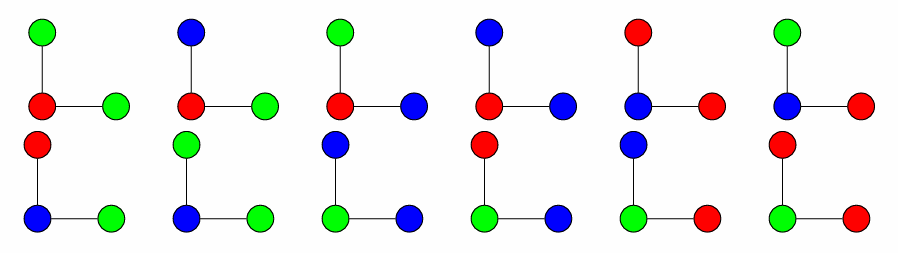
\includegraphics[width=0.8\linewidth]{P5.png}
    \label{fig:3-color-graph}
\end{figure}

\subsection*{Problem 6 (Extra Credit: 10 pts)}
Given a directed graph $G$ with $n$ vertices $V = \{1,2,\cdots,n\}$ and $m$ edges. We say that a vertex $j$ is reachable from $i$ if there is a directed path from $i$ to $j$. Design an $O(m+n)$-time algorithm (show the pseudo-code) that for any vertex $i$ outputs the smallest label reachable from $i$. For example, given the following graph you should output 1,2,2,2,1 corresponding to the smallest indices reachable from vertices 1,2,3,4,5 respectively.
\begin{figure}[H]
    \centering
    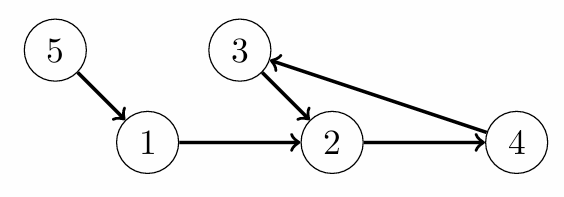
\includegraphics[width=0.5\linewidth]{P6.png}
    \label{fig:P6}
\end{figure}

\end{document}